
\documentclass[tikz,border=2pt]{standalone}
% Transformer styles for extended PlotNeuralNet figures
% Auto-generated initial version
\usepackage{tikz}
\usetikzlibrary{calc,fit,arrows.meta,positioning,backgrounds}

% Base styles (parameterized width/height usage: style=blk=<w>cm/<h>cm)
\tikzset{
  >={Latex[length=2mm]},
  blk/.style 2 args={draw,rounded corners=2pt,thick,fill=gray!10,minimum width=#1,minimum height=#2,align=center},
  sblk/.style 2 args={draw,rounded corners=2pt,thick,fill=gray!5,minimum width=#1,minimum height=#2,align=center,font=\scriptsize},
  % addnode expects diameter passed twice (w/h) for interface consistency
  addnode/.style 2 args={draw,circle,thick,inner sep=0pt,minimum size=#1,fill=white},
  tag/.style={draw,rounded corners=2pt,thin,fill=white,font=\scriptsize,inner sep=1pt},
  tagnode/.style 2 args={draw,rounded corners=2pt,thin,fill=yellow!15,minimum width=#1,minimum height=#2,align=center,font=\scriptsize},
  lane/.style={draw,rounded corners=3pt,thick,dashed,inner sep=6pt},
  gbox/.style={draw,rounded corners=4pt,thick,inner sep=6pt,fill=none},
  conn/.style={-Latex,thick},
  dashconn/.style={-Latex,thick,dashed},
}

\begin{document}
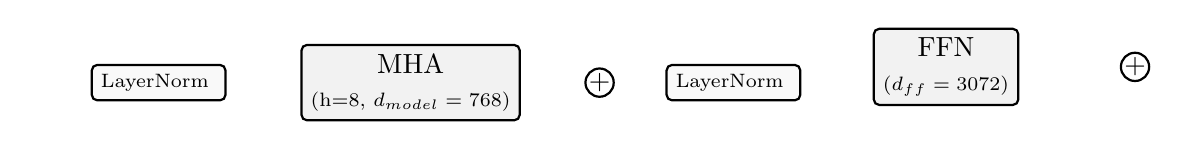
\begin{tikzpicture}

  \node[sblk=2.60cm/0.60cm] (ln1) at (0.00cm,0.00cm) { LayerNorm };

  \node[blk=3.80cm/1.20cm] (mha) at (3.20cm,0.00cm) { MHA\\\scriptsize(h=8, $d_{model}=768$) };

  \node[addnode=0.22cm/0.22cm] (add1) at (5.60cm,0.00cm) { + };

  \node[sblk=2.60cm/0.60cm] (ln2) at (7.30cm,0.00cm) { LayerNorm };

  \node[blk=3.20cm/1.20cm] (ffn) at (10.00cm,0.20cm) { FFN\\\scriptsize($d_{ff}=3072$) };

  \node[addnode=0.22cm/0.22cm] (add2) at (12.40cm,0.20cm) { + };


  
  \path[conn] (ln1.east) -- (mha.west);

  
  \path[conn] (mha.east) -- (add1.west);

  
  \path[conn] (add1.east) -- (ln2.west);

  
  \path[conn] (ln2.east) -- (ffn.west);

  
  \path[conn] (ffn.east) -- (add2.west);

  \path[conn] (ln1.west) -- ++(-0.80cm,0.00cm) |- (add1.north);

  \path[conn] (ln2.west) -- ++(-0.80cm,0.00cm) |- (add2.north);

\end{tikzpicture}
\end{document}